\chapter[Experiments]{Experiments}

The LPUS system is capable of doing many things. In this chapter, we list the
experiments that we took with LPUS and their results.

\section[Overview of what LPUS can do]{Overview of what LPUS can do}

The Windows kernel has global variables to control the system. LPUS can read
these global variables directly and collect the system information. In Section
7.2, we show how LPUS reads global variables to get the system information.
LPUS can perform pool tag scanning on both paged and non-paged pools, but
scanning with paged pool is more sophisticated as pages must be in RAM before
accessing. In Section 7.3, we show how LPUS performs pool tag scanning in the
non-paged pool region. Information collected will be further used for analysis,
especially finding hidden malware. In Section 7.4, we show how LPUS aggregates
collected information to apply malware detection.

\section[Using global variables]{Using global variables}

LPUS can get the global lists as described in Section 2.2.4, but in theory,
LPUS can access any global variables given the offset from the kernel base
address.  Many variables are not documented by Windows, to use these variables,
one must know the type and value they hold. Any individual having in-depth
knowledge in the Windows Internals will be benefited by using LPUS. In Table
\ref{tab:globalvars}, we list a few other kernel variables in Windows 7 and the
value they represent. Keep in mind that LPUS can access any kernel variable,
but a deep understanding of what the variables hold is required if we want to
use them to get the system information.

\begin{table}[t]
\centering
\begin{tabular}{ll}
\hline
  Global variable               \\ \hline
  MmPhysicalMemoryBlock         \\
  MmSystemRangeStart            \\
  MmHighestPossiblePhysicalPage \\
  MmPfnDatabase                 \\
\hline
\end{tabular}
\caption{Some kernel global variables}
\label{tab:globalvars}
\end{table}

Right now, LPUS only uses the variables that holds the pointer to lists of
process \texttt{PsActiveProcessHead}, \texttt{KiProcessListHead},
\texttt{HandleTableListHead}, the list of kernel modules
\texttt{PsLoadedModuleList}, the list of unloaded drivers
\texttt{MmUnloadedDrivers}, and the SSDT table \texttt{KiServiceTable}.  LPUS
listing the SSDT can be seen in Figure \ref{fig:ssdt_lpus}. LPUS listing the
unloaded drivers can be seen in Figure \ref{fig:unloaded_lpus}.

\begin{figure}[h]
  \centering
  \caption{LPUS lists the SSDT}
  \label{fig:ssdt_lpus}
  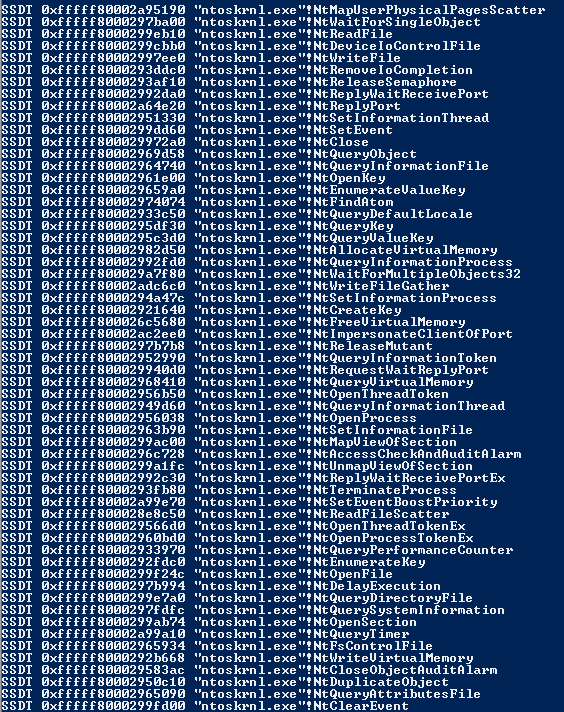
\includegraphics[scale=1]{images/ssdt_lpus.png}
\end{figure}

\begin{figure}[h]
  \centering
  \caption{LPUS lists the unloaded drivers}
  \label{fig:unloaded_lpus}
  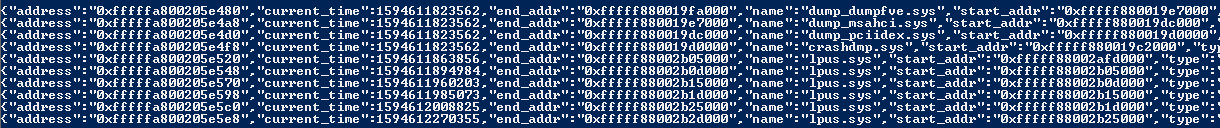
\includegraphics[scale=0.6]{images/unloaded_lpus.png}
\end{figure}

\section[Pool tag scanning]{Pool tag scanning}

LPUS supports a module to do pool tag scanning on the non-paged pool region.
Rekall on Section 3.2.3, the non-paged pool region can be accessed from the
kernel base by traversing the kernel structure as described in Table
\ref{tab:nonpaged}.  LPUS follows the table and gets the start and end of the
non-paged pool region.  The scan is performed page by page. If a page is
invalid, it is skipped. On every page, LPUS checks incrementally every
four-byte looking for the tag provided. If the tag matches, LPUS will check the
header for pool type and block size. A valid block must have the pool equal to
2 (enumeration of the non-paged pool), and the size must be larger than the
structure being found.  The search on the non-paged pool done by LPUS is
illustrated in pseudocode in Listing \ref{lst:poolscan}.

\begin{lstlisting}[language=cpp,caption={Pool Scan},label={lst:poolscan},float,floatplacement=H]
// Driver code
PVOID scan(ULONG64 startAddress, ULONG64 endAddress, ULONG tag) {
    POOL_HEADER p;
    PVOID currentAddr = (PVOID)startAddress;
    while (true) {
        if ((ULONG64)currentAddr >= endAddress)
            break;

        if (!MmIsAddressValid(currentAddr)) {
            currentAddr = (PVOID)((ULONG64)currentAddr + PAGE_SIZE);
            continue;
        }
        if (!MmIsAddressValid((PVOID)((ULONG64)currentAddr + 0x10))) {
            // >> currentAddr is at the end of a page,
            //    currentAddr+0x10 is a bad page
            //    which if we parse the header, will crash
            currentAddr = (PVOID)((ULONG64)currentAddr + 0x4);
            continue;
        }
        currentAddr = (PVOID)((ULONG64)currentAddr + 0x4);

        toPoolHeader(&p, (PVOID)currentAddr);
        if (p.poolType != 2) continue;
        if (p.tag != tag)
            continue;

        return p.addr;
    }
    return (PVOID)endAddress;
}

// User application code
// repeatedly call scan
PVOID ptr = poolStart;
while (ptr != poolEnd) {
  ptr = scan(ptr, poolEnd, tag);
  if (ptr == poolEnd) break;
  POOL_HEADER block = (POOL_HEADER*) ptr;
  if (block->PoolSize * 16 < structSize) {
    ptr += 0x4;
    continue;
  }
  // === the block is valid ===
  // parse data in block
  // ==========================
  ptr += block->PoolSize * 16;
}

\end{lstlisting}

Paged pool can also be scanned, in Windows 7 there are two variables showing
where the paged pool is, \texttt{MmPagedPoolEnd} and
\texttt{MmSizeOfPagedPoolInBytes}. \texttt{MmPagedPoolEnd} holds the end of the
paged pool and \texttt{MmSizeOfPagedPoolInBytes}. We can easily find the start
and end of the paged pool. However, scanning in this paged pool is more
complex.  The paged pool does not always reside in the physical memory, and
they will be paged out if not needed. To prevent this, we have to \textit{lock}
the page inside the memory first. This can be done by calling
\texttt{MmProbeAndLockPages}.  After locking the page, we can access the memory
as usual. There is another aspect we must pay attention to, the page validity.
This paged pool range is vast, many pages may not be valid and will trigger
exception on access. In theory, the paged pool can be scanned, but we have not
implemented the feature.  One big reason why we chose not to implement this
feature is that most important Windows objects allocation are located inside
the non-paged pool, there is no reason to scan the paged pool if the
information found is limited or none.

The LPUS module implementing pool tag scanning returns the block address on any
block matches the criteria. For ordinary objects without headers, by skipping
the \texttt{\_POOL\_HEADER}, we get the address to the object. For executive
objects, which have headers around them, it is harder to get the object's
address. We currently check the member fields for validity, e.g., for
\texttt{\_EPROCESS} and \texttt{\_ETHREAD}, we check the \texttt{CreateTime} to
be between the OS boot time and scan time. We have implemented pool tag
scanning for \texttt{\_EPROCESS}, \texttt{\_ETHREAD},
\texttt{\_DRIVER\_OBJECT}, \texttt{\_LDR\_DATA\_TABLE\_ENTRY},
\texttt{\_FILE\_OBJECT}. LPUS can also scan objects related to internet
connections, kernel callbacks, and mutexes, but we have difficulty implementing
these objects and leaving them for future development.

The results of pool tag scanning for \texttt{\_EPROCESS} and \texttt{\_ETHREAD}
can be seen in Figure \ref{fig:psxview}, where we demonstrate LPUS comparing
the processes found by list walking and scanning.

\begin{figure}[h]
  \centering
  \caption{LPUS compare lists of process}
  \label{fig:psxview}
  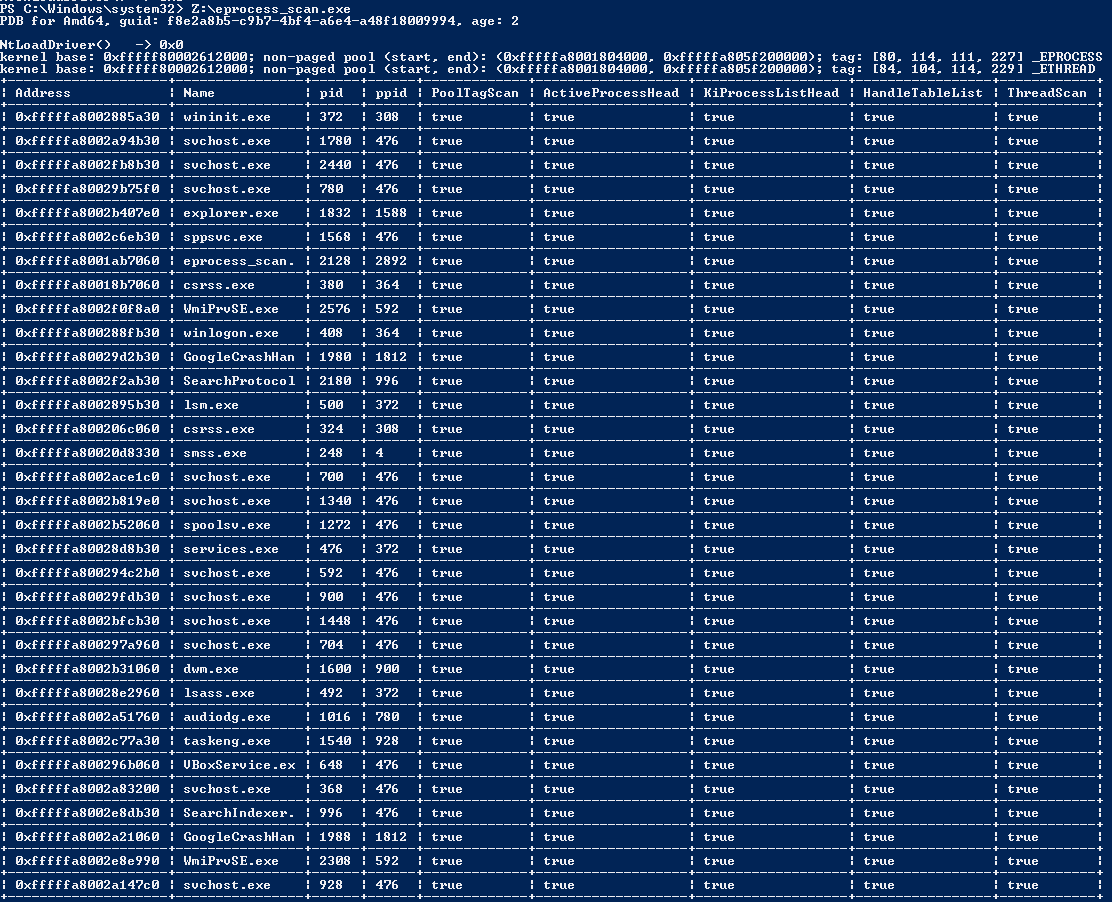
\includegraphics[scale=0.7]{images/psxview.png}
\end{figure}

\section[Driver's IRP listing]{Driver's IRP listing}

LPUS supports IRP hooking detection by inspecting the driver list
\texttt{MajorFunction}. To do this, LPUS will first scan for
\texttt{\_DRIVER\_OBJECT} and \texttt{\_LDR\_DATA\_TABLE\_ENTRY} and saves the
results into two list, drivers and modules. When the user chose a driver to
inspect the \texttt{MajorFunction}, LPUS will loop through each function
pointer in the \texttt{MajorFunction} list and search for the module containing
the function. Figure \ref{fig:irp_lpus} is the sample results of LPUS when
inspecting a driver object at a specific address.

\begin{figure}[h]
  \centering
  \caption{LPUS inspects the IRP of a driver}
  \label{fig:irp_lpus}
  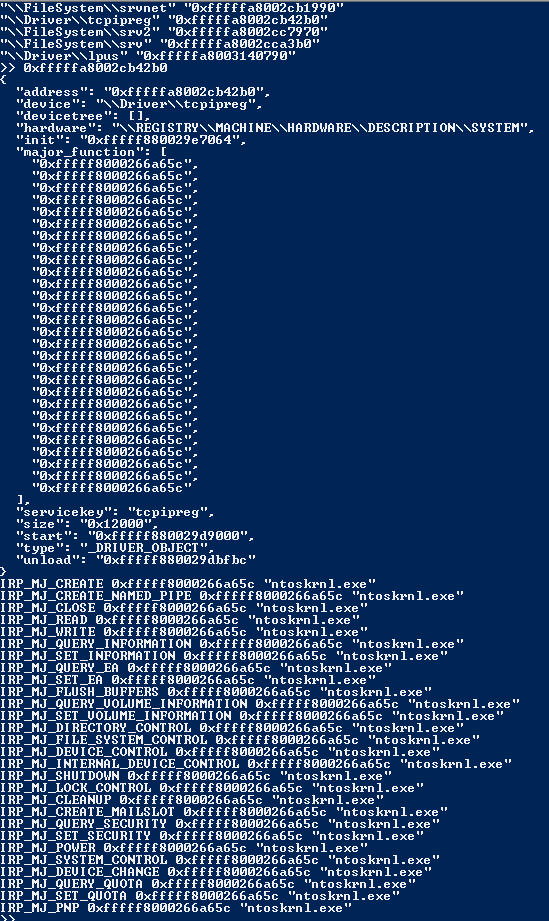
\includegraphics[scale=1]{images/irp_lpus.png}
\end{figure}

% Compared to using WinDbg
% where the machine has to be stoped LPUS is a better option. WinDbg supports
% live mode by loading a special kernel driver when the system loads and requires
% the user to enable debug mode, LPUS can work without these requirements and can
% still query the kernel system.

\section[Comparing LPUS]{Comparing LPUS}

In this section, we compare LPUS with Volatility. We set up the test
environment as follows. Run an instance of Windows 7 SP1 64-bit in Virtual Box.
Connect WinDbg to debug the OS. Run LPUS and output the results into a JSON
file.  Immediately after LPUS terminates, pause the system with WinDbg. In
WinDbg use the \texttt{.dump /f} command to generate a full kernel dump, full
RAM contents. After WinDbg finishes, use \texttt{VBoxManage}, a utility to
manage machine instances in Virtual Box, to output the RAM content. With the
two memory files, one from WinDbg and one from Virtual Box, we run Volatility
commands to get the same information as LPUS. We then use a Python script to
compare LPUS output with the Volatility results using the WinDbg memory file,
and Volatility results using the Virtual Box memory file. The results are
compared using the object's addresses. In Table \ref{testinfo}, we list the
information to compare on the Volatility command to get the information. In
Table \ref{testresult}, we have the results of the comparison.


\begin{table}[t]
\centering
\begin{tabular}{ll}
\hline
  Information         & Volatility command \\ \hline
  Process list        & pslist             \\
  Process scan        & psscan             \\
  Threads             & threads            \\
  Thread scan         & thrdscan           \\
  Kernel modules      & modscan            \\
  Kernel module scan  & modscan            \\
  Drivers             & driverscan         \\
  Unloaded drivers    & unloadedmodules    \\
  SSDT                & ssdt               \\
\hline
\end{tabular}
\caption{Test information and Volatility command}
\label{tab:testinfo}
\end{table}


\begin{table}[t]
\centering
\begin{tabular}{lrrrr}
command         & common & LPUS only & WinDbg only & VBox only \\
\hline
driverscan      & 105    & 2         & 1           & 1         \\
modscan         & 67     & 0         & 71          & 71        \\
modules         & 137    & 1         & 0           & 0         \\
pslist          & 39     & 1         & 0           & 0         \\
psscan          & 0      & 41        & 0           & 0         \\
thrdscan        & 0      & 41        & 0           & 0         \\
threads         & 574    & 16        & 4           & 23        \\
unloadedmodules & 4      & 0         & 1           & 1         \\
ssdt            & 390    & 11        & 836         & 836       \\
\hline
\end{tabular}
\caption{Test results}
\label{tab:testresult}
\end{table}
